\chapter{Contributions to Spot}

This chapter present the different things I have done on Spot during the internship. Might it be
some algorithms implemented, scripts, display arrangements, benchmarks, results analyzes, etc.

\noindent All the achieved work is presented in a chronological way, to bring out the difficulties
encountered, the unexpected results that had influence on the advancement of the work.

\section{fastSAT}
As a quick reminder, here are the required characteristics for the SAT solver:
\begin{itemize}
 \item licence compatibility with Spot's one (GNU GPL v3),
 \item simplicity of integration for future updates,
 \item effectiveness.
\end{itemize}

\noindent The project \textbf{fastSAT}\cite{5} was born to help choose the SAT solver to distribute with
Spot. Until now, SAT-based minimization was performed through an external SAT solver. The default one
was Glucose \cite{12} (3.0 version). Therefore, it seems logical to consider Glucose as a possible
candidate. \textbf{fastSAT}\cite{5} compared Glucose 4.0 \cite{12} to CryptoMiniSat 5.0.1\cite{20} and
PicoSAT 965 \cite{21}. Note that some SAT solvers provide two versions, one parallal and one simple
essentially because of the SAT competitions. In short, were compared:
\begin{itemize}
 \item Glucose syrup (parallal) 4.0
 \item Glucose simple 4.0
 \item CryptoMiniSat parallal 5.0.1
 \item CryptoMiniSat simple 5.0.1
 \item PicoSAT 965
\end{itemize}

The next three figures (\ref{fig:satchoose_1}, \ref{fig:satchoose_2} and \ref{fig:satchoose_3}) show some
comparaisons for three formulas. About twenty formulas have been tested in two modes: by forcing the number
of state and by doing the complete cycles of minimization. It has been executed on a computer with an
\textbf{Intel(R) Core(TM) i7-4710HQ CPU @ 2.50GHz} processor and  a \textbf{8 GiB} system memory.
The measuring tool used is the open Google Benchmark tool \cite{21}.

\begin{figure}[H]
 \centering
 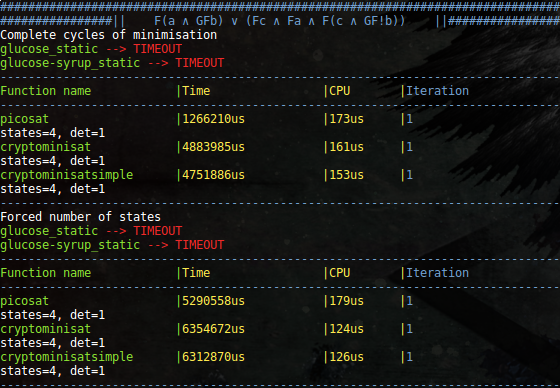
\includegraphics[scale=0.7]{img/satchoose_1.png}
 \caption{Benchmark for formula $F(a \land GFb) \lor (Fc \land Fa \land F(c \land GF(!b)))$}
 \label{fig:satchoose_1}
\end{figure}

\begin{figure}[H]
 \centering
 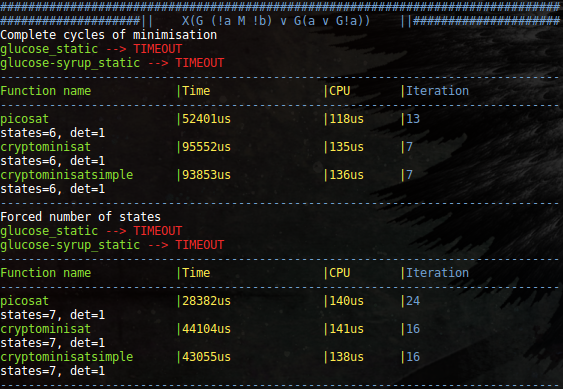
\includegraphics[scale=0.7]{img/satchoose_2.png}
 \caption{Benchmark for formula $X(G (!a M !b) \lor G(a \lor G(!a)))$}
 \label{fig:satchoose_2}
\end{figure}

\begin{figure}[H]
 \centering
 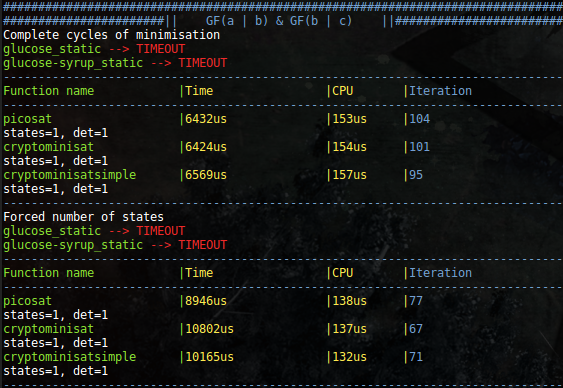
\includegraphics[scale=0.7]{img/satchoose_3.png}
 \caption{Benchmark for formula $GF(a \lor b) \land GF(b \lor c)$}
 \label{fig:satchoose_3}
\end{figure}

\noindent In conclusion, among the different SAT solvers, \textbf{PicoSAT} was choosen for its strong
performances. It consists of two source code files: \textbf{picosat.h} and \textbf{picosat.c} and was
easily integrated and harmonised with Spot.

\textbf{fastSAT}\cite{5} project is fully availlable and anyone can reproduce the benchmarks. Feel free to
have a look.

\section{New Satsolver class}
There was already a satsolver class that is instantiated at the beginning of the SAT-based minimization
procedures, formerly used to initialize a temporary \textbf{cnf file} (DIMACS \cite{18}) and return
it. The file writing was directly made by those procedures.

\noindent The objective is to completely abstract the file writing. SAT-based minimization procedures will
just have to instantiate a satsolver object at the beginning and make calls to its functions. Thoses
functions will call the SAT solving library functions. But as we still want to support any external
satsolver, this class must continue to handle temporary \textbf{cnf files}.\\

\begin{figure}[h]
  \centering
  \begin{tikzpicture}
    \begin{umlpackage}{Pseudo UML}
     \umlclass[name=satsolver, template=T]{spot::satsolver}
     {
       psat\_ : PicoSAT*\\
       cnf\_stream\_ : std::ostream*\\
       nb\_clauses\_ : int\\
       nb\_vars\_ : int\\
       ...
       }{
       add(std::initializer\_list\textless int\textgreater values : void\\
       add(int v) : void\\
       comment(T first, Args... args)\\
       get\_nb\_clauses() : int\\
       get\_nb\_vars() : int\\
       get\_solution() : std::pair\textless int, std::vector\textless bool\textgreater\textgreater\\
       ...
     }
    \end{umlpackage}
  \end{tikzpicture}
  \caption{Satsolver class UML representation}
  \label{fig:sat_uml}
\end{figure}

\noindent The figure \ref{fig:sat_uml} shows a pseudo UML representation of the new satsolver class. It can either
initialize PicoSAT or a cnf\_stream\_. The idea is to let its function (add, comment, etc.) to decide
if they call PicoSAT functions or write in the cnf\_stream\_. That way, SAT-based minimization procedures
are not aware of what's going on behind and can repeat over and over again the same algorithms.\\

\noindent Of course the clause counting mechanism is provided by the new satsolver class. At the end,
SAT-based procedures will just have to call the \textit{get\_solution()} method.\\

Once this was done, SAT-based procedures had already gained some speed. For instance, with this command
line:
\begin{lstlisting}[language=bash,caption={bash command-line to test a formula minimization using ltl2tgba}]
  time ltl2tgba -D -x sat-minimize 'G(a -> Fb) & G(c -> Fd)'
                        --stats='states=%s, det=%d’
\end{lstlisting}
we obtained:\\\\
\begin{tabular}{|c|c|}
 \hline
 Version & Result\\
 \hline
 PicoSAT as linked SAT solving library&0.29s user 0.08s system 98\% cpu 0.371 total\\
 PicoSAT as external SAT solver&0.82s user 0.09s system 98\% cpu 0.925 total\\
 \hline
\end{tabular}
